\section{Motivations and Foundations}\label{sec:foundationMotivation}
In this section, we describe the motivation and foundations of our work. More specifically, we present the context of our work in \secref{context}. \secref{requirements} describes the requirements that we have used when assessing related works in the literature. In \secref{relatedWork}, we describe related works and how they are failing to satisfy our requirements. Finally, \secref{illustratingScenario} describes an illustrating scenario that we use throughout this paper.  

\subsection{Context}\label{sec:context}
This work takes place in a private collaboration between the Orange and the french laboratories LAAS and IRIT. It revolves around the \thingin\footnote{\url{https://hellofuture.orange.com/en/thingin-the-things-graph-platform/}, last accessed 7 December 2019} platform whose aim is to maintain thorough structural and semantic description of the environments, such as cities or buildings, containing objects that may be inter-related between themselves. While \thingin is based on NGSI-LD\footnote{\url{https://www.etsi.org/newsroom/press-releases/1519-2019-01-etsi-cim-group-releases-full-feature-specification-for-context-information-exchange-in-smart-cities}},on a high-level information model, it supports import and export RDF data.

\figref{contextThingIn} shows the positioning of \thingin in an Internet of Things (IoT) ecosystem. In such an ecosystem, there are objects of different kinds such as \kword{IoT devices} (e.g. sensors, actuators) and \kword{non-connected objects} (e.g. tables, chairs) . For multiple reasons, such as different protocols, standards, there is a heterogeneity of \kword{IoT platforms} for managing  devices. Consequently, there may be no single entrypoint to access description of objects. In this situation, \thingin can homogenize access to these descriptions by acting as a directory of objects.

\begin{figure}[h]
	\centering
	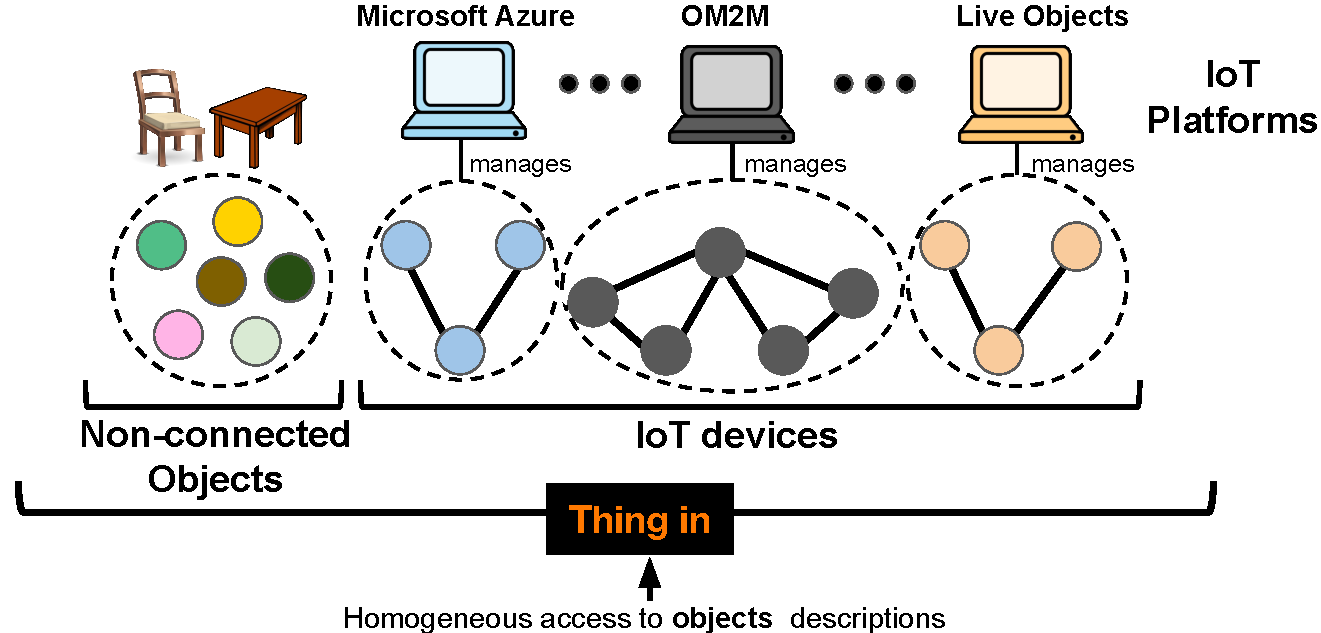
\includegraphics[scale=0.5]{images/contextThingIn.pdf}
	\caption{\thingin in an IoT ecosystem}
	\label{fig:contextThingIn}
\end{figure}

For \thingin to be used as a catalog of objects, it must contain their descriptions. However, importing these descriptions into it is problematic as they are heterogeneous due to the diversity of data formats and domain models that exist. As mentioned above, \thingin can import data in RDF. This is where the task of facilitating the transformation of heterogeneous semi-structured data to RDF comes into play.



\subsection{Requirements}\label{sec:requirements}
Before moving on to related works, let us explicitly mention the requirements used when considering these works. We require that an approach:

\paragraph{\textbf{R1. does not necessitate prior knowledge of existing ontologies}} There may be numerous ontologies usable to describing a particular raw data. An approach should not depend on this knowledge but throughout the mapping process, it provides the user with information to use a particular ontology. 

\paragraph{\textbf{R2. generate initial mappings that can be customized}} To re-enforce the first requirement, generated mappings should be provided as an entrypoint to start identifying the potential ontology entities that may be used. 


\paragraph{\textbf{R3. does not restrict the data modeling aspect}} The approach should not force a particular data modeling decision. For example, an approach should not force the use of only ontology data properties to model the properties (e.g. \kword{TOTAL}) in \rawData.

\paragraph{\textbf{R4. Maximize the reuse of existing ontologies for describing the raw data}} The approach should not require creating new ontology entities to model the raw data while respecting the semantics of the reused ontologies. 

\paragraph{}We believe that the above requirements are the minimum necessary conditions to facilitate the RDFization of heterogeneous semi-structured data. Let now use these requirements and proceed to the related works in the next section. 

\subsection{Related Works}\label{sec:relatedWork}

%\subsection{Related Work}\label{sec:relatedWorks}



%criteria:
%-knowledge of ontologies
%-data modeling
%-no initial mappings

%mapping language
%=================
%- thick knowledge stack
%	- 
	
%Mapping Language (implicit or explicit)
%----------------------------------------
%Facilitate the transformation of raw data to RDF, but user must have a knolewdge of the ontologies they want to
%use
%- R2RML~\cite{R2RML_W3C:12}
%" r2rml[3]  is  thew3c -recommended language to dene mappings to generaterdf from data derived from relational databases"

%- RML~\cite{dimou2014rml}
%"generation of data inrdf representation based on multiple heterogeneous data sources, e.g.,xmlandjson"
%- XSPARQL
%- GRADDLE
%- SPARQL Generate
%- Direct Mapping 




%some lines
%Semi-Automatic
%---------------
% LOVER -http://ansgarscherp.net/publications/pdf/W24-SchaibleEtAl-LOVER-SupportForModelingDataUsingLinkedOpenVocabularies.pdf
%- Datalift [1]
%- LodRefine [2,Sec.2]
%- Sheet2RDF~\cite{fiorelli2015sheet2rdf}
%Must specify a subject
%Must annotate each header with rdf schema
%"Next, the mappings are complemented with data fractions from the databases.sheet2rdf[10] is a platform that uses apearl[11 ] document to map data in spreadsheets tordf. Itsgui allow users to view the source data, define the mappings by editing thepearl document directly, and view the resulting rdf through a tabular-structure. However, the adoption of the tool decreases because users need knowledge aboutpearl to edit the mappings"
%- RML Editor
%- chatbots

We expect from an automatic tool to transform semi-structure data to RDF, the following
requirements:
\begin{enumerate*}[label={\alph*)},font={\bfseries}]
	\item \emph{Data modeling}: the user do not have to care how the data should be 
	modelised. That is to say, if he should modelise columns as class or properties.
	\item \emph{No prior knowledge on ontologies}: the end-user should not need to
	know which ontologies he should use to modelised his data, nor how to use the 
	ontologies.
	\item \emph{No initial mapping}: to transform his data the end-user only need to
	provide a raw data. However, he can enhance the transformation by provinding
	simple keywords about columns.
\end{enumerate*}


Many works have been done to help end-user to transform raw data in RDF data. 
We can split those work into
two main categories. The mapping languages and semi-automatic approches.

\paragraph{Mapping languages} aims at ease the transformation process. R2RML~\cite{R2RML_W3C:12} is a mapping
lanaguage to transform relational database to RDF data and is a recommendation from the W3C. 
RML~\cite{dimou2014rml} enhance the previous approach by handling heterogenous data sources in entry of the
transformation process and is subject centric. SPARQL-GENERATE~\cite{lefranccois2016flexible} allow the
transformation of heterogenous data sources and previous transformation operation on the original dataset.
However, all of those approches do not fulfill our requirements.
Indeed, they are only a step in the transformation process.
Our vision of transforming semi-structured data to RDF is broader and take also in consideration the
assistance to create the mappings.

\paragraph{Semi-Automatic approches} go one step futher compared to mapping languages, because they assist
the user during the mapping process. The approach Sheet2RDF\cite{fiorelli2015sheet2rdf} propose both
a command line tool and a user interface tool. However, to use this approach a prior knowledge about
PEARL~\cite{pazienza2012pearl} mapping is required. Therefore it do not fulfill or \emph{Data Modeling}
requirement.

RMLEditor~\cite{heyvaert2016rmleditor} is a graphical interface for RML~\cite{dimou2014rml}. 
It has two modes, one without the editor, where the end-user have to import the raw data and the RML mapping.
A second mode where the end-user do not need to have prior knowledge about the mapping language's
specification. Nevertheless, in both scenarios the end-user need to provide initial
mappings, which do not complies with our requirements.

% "context information about the dataset which has to be modeled as Linked Data"
% By using the Swoogle API for a search based on exact string match
% as it is important to get the list of elements which are supposed to be mapped to classes and properties from existing vocabularies
LOVER~\cite{schaible2013lover} it provides the ontology engineer search mechanism for
classes and properties with metadata about classes and properties and
usage example. In a step of the transformation process, the ontologie engineer is 
supposed to enumerate the elements to be mapped, and if they have to be mapped to classes
or properties. Therefore, the end-user  need to have some knowledge in 
\emph{Data modeling}. Whereas, in our approach we want the modeling part to be 
transparent to the end-user.

% Open Refine
% rename or remove columns
% versionning of operations on the dataset
% sort, faceting, detecting duplicates, applying text filter, using simple cell transformation, removing matching rows
% reconcile our cell values with Freebase URLs two mode one for values already in freebase, one if columns values are not in freebase
% 
% Two types of reconciliation 1) value of cells are Freebase ids 2) Terms not related to freebase identifier (Freebase receonciliation service)
% Freebase reconciliation service propose 3 modes 1) decide against what type of records you want to reconsile (list)contacted the service with part of your data to try to guess the type of your column data
% reconciliation against type (the user choose), reconcile against no particular type -> find URL for each unique cell value and define best candidates
% 2) Auto-match candidate with high confidence 
% 3) allow to send additional information to de reconciliation service by considering several columns
% reconcile only on one dataset?
% reconciliation per cell value? "OpenRefine reconciled the value with a URL"
Open Refine~\cite{verborgh2013using} is a tool to transform semi-structured data where basic operations such as sorting data, detecting duplicates, applying text
filter, etc \dots can be performed. One of the operation that can be performed is to reconciliate data with an RDF dataset.
Several modes are possible to perform the transformation, but the aim is to reconciliate each individual cell values to existing URL
in the given dataset. Reconciliation is a way to transform raw data to RDF data but is different from generating mappings.
Indeed, reconciliation focus on individuals cells values, whereas mappings generation often consider the overall structure of the files.
Even if those two approaches can be complementary, reconciliation require to know pertinent real dataset.


% Reconciliation identifying multiple representations of the same real-world object
An RDF extension~\cite{maali2011re} is available for Open Refine~\cite{verborgh2013using}, where reconciliation against existing
databses is still available. In addition, the tool allow user to define a skeleton of mappings. But you have to define which
concepts to use and relation between terms. Whereas in our approach we want to assist the end-user in the creation of mappings.
However, reconciliation is complementary to our approach.


% our tool uses two knowl-edge graphs, DBpedia and YAGO, the ontologies of LOV
% from a set of instances of each column, our tool searches corresponding entities in DBpedia and YAGO
% saturate mapping with OL and RDFs eg ol:equivalentTo
Another approach is based on a chat-bot tool~\cite{moreau2019semi} wich can generate RDF mapping from structured data by asking simple question to the user.
It uses reconciliation against DBpedia and YAGO to infer classes of columns. Then it uses LOV~\footnote{\url{https://lov.linkeddata.es/dataset/lov/}}
to find properties. To confirm choices it ask the user to answer simple queries. Even if this approach requires no knowledge in RDF and Data Modeling
it is limited by the reconciliation phase. Indeed, firstly there is, currently, only two datasets against which the reconciliation can be performed. Secondly,
it makes the hypothesis that a matching URIs will be find, which will not be possible on geonames~\footnote{\url{https://www.geonames.org/}} 
for example, such as all URIs are random numbers.

DataLift~\cite{scharffe2012enabling} is a platform to publish linked data. It assist the user through the mapping generation and linkind dataset
step. However, as mentionned by the authors, the user needs knowledge in the Semantic Web (RDF, RDFS/OWL and SPARQL).

Karma

Juma
\subsection{Illustrating Scenario}\label{sec:illustratingScenario}
In our project, we are using \thingin in an IoT context. However, due to the project's bindings, we cannot publish descriptions of objects in use. For illustration purposes, so as to use any synthetic data, we consider a parking dataset\footnote{\url{http://data.metropolegrenoble.fr/ckan/dataset/parkings-de-grenoble/resource/a6919f90-4c38-4ee0-a4ec-403db77f5a4b}, last accessed on 7 December 2019} from Grenoble open data portal\footnote{\url{http://data.metropolegrenoble.fr/}, last accessed on 7 December 2019}. \figref{sampleRawData} is part of a preview of that dataset taken directly from the data portal.

In the parking dataset, there may be several columns that may be \colorbox{yellow}{little to no use}\coment{fano}{?} for external users. For example, \kword{\_id} may be contain data for an internal use, \kword{CODE} contain the same information as \kword{id} and \kword{TYPE} and \kword{type} contain the same information that may not meaningful.

\begin{figure}[h]
	\centering
	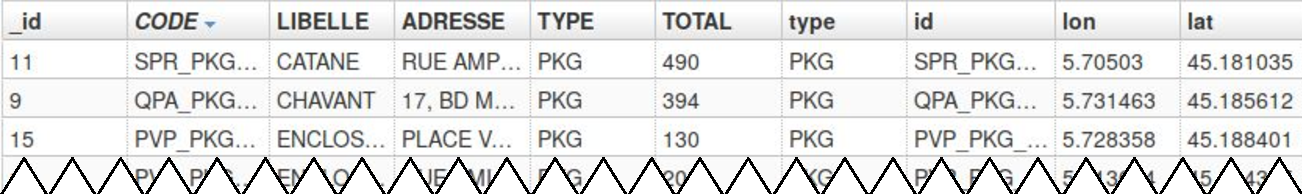
\includegraphics[scale=0.45]{images/sampleRawData.pdf}
	\caption{Parking data from Grenoble Open Data Portal}
	\label{fig:sampleRawData}
\end{figure}

\figref{sampleOntologyRawData} shows a possible vocabulary, that we refer to as a final mapping, for describing the parkings in \figref{sampleRawData}. The light blue and orange arrows are data and object properties respectively. As we can see, the final mapping reuses terms from several ontologies. The prefixes in the IRIs of ontology entities are shown in \reftab{prefixList}. Throughout this document, we use prefixes from this table. Also, below the IRIs of most ontology entities in \figref{sampleOntologyRawData}, the green labels refers to schema elements (i.e. column headers) in the parking data (\cf \figref{sampleOntologyRawData}) and above them is the ontology entity to which they have been mapped.

In our approach, formally described in \secref{approach}, the final mapping contains at least a class to type objects in the raw data and ontology entities that describe  objects' properties. For example, in \figref{sampleOntologyRawData}, we use \kword{mv:ParkingFacility} to type the objects in \figref{sampleRawData} and, the data property \kword{wgs84:long} and class \kword{mv:Capacity} are used to model their \kword{lon} and \kword{TOTAL} property respectively. Additionally, the latter ontology entities must be related to the latter classes used for typing directly or indirectly via other ontology entities. \kword{wgs84:long} is directly related as its domain include \kword{mv:ParkingFacility}. \kword{wgs84:long} can be used directly to specify the values as its domain include \kword{mv:ParkingFacility}. Nevertheless, for \kword{mv:Capacity}, the final mapping includes \kword{mv:capacity} to link to \kword{mv:ParkingFacility} and the data property \kword{mv:maximumValue} to specify the values.  



\begin{comment}
To express the values of the object's properties in the raw data, we use data properties or classes that are in the domain of a data property. For example, in \figref{sampleOntologyRawData}, \kword{lon} is modeled using the data property \kword{wgs84:long} that is used to specify the \kword{lon}'s values. Also, \kword{TOTAL} is modeled using the class \kword{mv:Capacity}. This class is the domain of the data property \kword{mv:maximumValue}.Therefore, the data property is used to specify the \kword{TOTAL}'s values. Moreover, \kword{wgs84:long} has been used as it is in the domain of \kword{mv:ParkingFacility}. Also, \kword{mv:capacity} is added to the \descriptionVocabulary as it relates \kword{mv:ParkingFacility} to \kword{mv:Capacity}.
\end{comment}

%Additionally, in our approach, the \descriptionVocabulary must be coherent. 

%More explicitly, entities in \descriptionVocabulary to represent the relation between the type and considered entities. 



\begin{figure}[h]
	\centering
	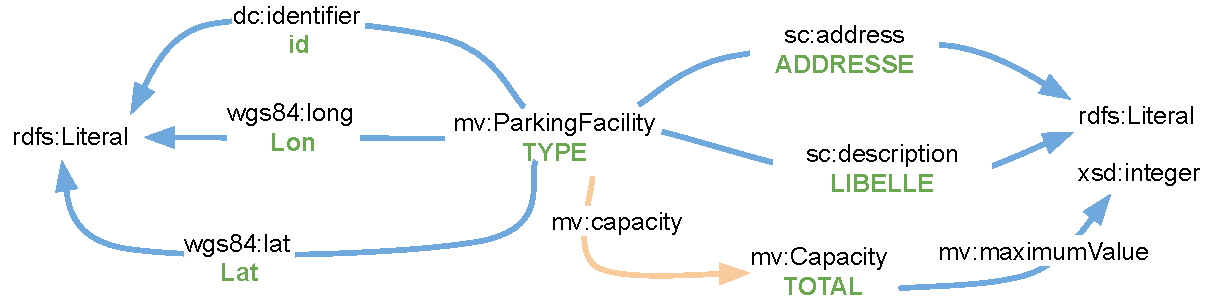
\includegraphics[scale=0.5]{images/sampleOntologyRawData.pdf}
	\caption{Vocabulary to describe parking data}
	\label{fig:sampleOntologyRawData}
\end{figure}
%The parking description reflects some important design decisions in our approach. First, as we can see, 

\begin{table}[]
	\centering
	\begin{tabular}{|l|l|l|}
		\hline
		\textbf{Prefix} & \textbf{Vocabulary Name} & \textbf{Namespace IRI}                       \\ \hline
		xsd             & XML Schema Definition    & http://www.w3.org/2001/XMLSchema\#           \\ \hline
		rdfs            & RDFS                     & http://www.w3.org/2000/01/rdf-schema\#       \\ \hline
		owl				& Web Ontology Language    & http://www.w3.org/2002/07/owl\#               \\ \hline
		sc              & Schema.org               & http://schema.org/                           \\ \hline
		mv              & MobiVoc                  & http://schema.mobivoc.org/                   \\ \hline
		
		wgs84           & WGS84                    & http://www.w3.org/2003/01/geo/wgs84\_pos\#   \\ \hline
		dc           & Dublin Core Metadata Terms                    & http://purl.org/dc/terms/   \\ \hline
		ign           & IGN administrative units                    & http://data.ign.fr/def/topo   \\ \hline
		
	\end{tabular}
	\caption{List of Vocabulary Prefixes}
	\label{tab:prefixList}
\end{table}